% Issue #75; owner: Bytebard089. Input from reports/phase2/main.tex.
% Numbers: results/metrics/fd001_ablations{,_paired,_seeds}.csv and
% results/figures/fd001_ablations.png, from notebooks/phase2/11_ablations.ipynb (#69).
% Table: tables/ablations.tex (generated from the same CSVs).

\section{Ablation Studies}
\label{sec:ablations}

Hybrid A combines several design choices: a 30-cycle window, a training cap
of 125, five groups of engineered features, a learned gate between a sequence
branch and a feature branch, and an MSE loss. An \emph{ablation} changes one
of these choices, keeps every other setting fixed, and measures the effect.
This section asks what each choice contributes and answers the question the
project brief leaves open: does a model that reads longer history predict
better, and at which stage of an engine's life?

\subsection{Method}
Each variant starts from the final Hybrid A configuration and changes one
setting. Six groups are tested: window length (15, 30, 60 and 90 cycles);
training cap (none, 100, 125 and 150); feature groups in the feature branch
(all; all but age; age and current sensors only; rolling statistics only);
the cycle index as an extra sequence input; the loss; and the branches
(sequence only, features only, plain concatenation, and the gate). The
asymmetric loss weights the squared error of a \emph{late} prediction, one
that promises more life than the engine has left, by $(13/10)^2\approx1.69$.
This is the ratio of the second-order terms of the NASA
score~\cite{Saxena2008damage}, whose late and early scales are 10 and 13.

Every variant is trained on the three engine-grouped folds of
Section~\ref{sec:dl_dataset} and scored with $\mathrm{RMSE}_{\leq K}$, $K=130$
(Section~\ref{sec:target_selection}). The official test set is not used. All
variants are trained with seed 42. The window and branch groups carry the
main conclusions, so they were repeated with seeds 43 and 44.

Each held-out engine is scored once per run, so two variants can be compared
engine by engine. The \emph{engine error} is the RMSE over one engine's
cycles with true RUL at most $K$. For each variant against the base, we
report the difference in RMSE over engines with a paired bootstrap 95\%
confidence interval (10{,}000 resamples of engines)~\cite{Efron1993introduction},
and a Wilcoxon signed-rank test on the engine errors~\cite{Wilcoxon1945individual}.
The 14 tests form one family under Holm's correction~\cite{Holm1979simple},
so the number of variants does not inflate false positives. For the
three-seed groups, both sides are averaged over seeds before the comparison.
A change counts as real only if its interval excludes zero \emph{and} its
corrected $p$ is below 0.05.

\begin{table*}[t]
\centering
\caption{Ablations of Hybrid A on FD001 (cross-validation, 3 folds). RMSE:
over engine errors, averaged over seeds. $\Delta$: variant minus base
(negative is better), paired bootstrap 95\% CI. $p_\mathrm{Holm}$: Wilcoxon
signed-rank, Holm-corrected over all 14 comparisons. Early ($100<y\leq K$),
mid ($50<y\leq100$) and late ($y\leq50$): RMSE over held-out cycles in each
life stage. The top block uses seeds 42--44, the bottom block seed 42.}
\label{tab:ablations}
\footnotesize
% Generated by scripts/prepare_ablations_table.py from
% results/metrics/fd001_ablations{,_paired,_seeds}.csv (#69). Do not edit by hand.
\begin{tabular}{@{}lccccccc@{}}
\hline
Variant & Seeds & RMSE & $\Delta$ [95\% CI] & $p_\mathrm{Holm}$ & Early & Mid & Late \\
\hline
\textbf{Base (Hybrid A)} & 3 & 16.61 & -- & -- & 19.39 & 20.06 & 9.62 \\
Window 15 & 3 & 16.63 & $+$0.02 [$-$0.17, $+$0.21] & 1.00 & 19.48 & 20.07 & 9.58 \\
Window 60 & 3 & 16.68 & $+$0.07 [$-$0.11, $+$0.26] & 1.00 & 19.54 & 20.22 & 9.44 \\
Window 90 & 3 & 16.67 & $+$0.06 [$-$0.12, $+$0.23] & 1.00 & 19.48 & 20.20 & 9.48 \\
Sequence branch only & 3 & 16.90 & $+$0.29 [$-$1.49, $+$2.19] & 0.20 & 15.88 & 21.69 & 11.10 \\
Feature branch only & 3 & 17.40 & $+$0.79 [$+$0.41, $+$1.18] & 0.051 & 20.08 & 21.29 & 9.79 \\
Concatenation, no gate & 3 & 16.92 & $+$0.31 [$-$0.03, $+$0.64] & 1.00 & 19.70 & 20.57 & 9.55 \\
\hline
\textbf{Base (Hybrid A)} & 1 & 16.82 & -- & -- & 19.41 & 20.47 & 9.70 \\
No cap & 1 & 31.14 & $+$14.32 [$+$11.26, $+$17.36] & $<$0.001 & 41.31 & 36.32 & 13.88 \\
Cap 100 & 1 & 15.69 & $-$1.13 [$-$2.33, $+$0.05] & 1.00 & 24.67 & 14.70 & 7.92 \\
Cap 150 & 1 & 19.97 & $+$3.15 [$+$1.91, $+$4.37] & $<$0.001 & 23.71 & 24.18 & 10.96 \\
Features: no age & 1 & 17.50 & $+$0.68 [$-$0.36, $+$1.72] & 0.70 & 19.14 & 21.52 & 10.81 \\
Features: current only & 1 & 16.29 & $-$0.53 [$-$2.41, $+$1.40] & 1.00 & 15.12 & 21.51 & 9.66 \\
Features: rolling only & 1 & 17.38 & $+$0.56 [$-$0.50, $+$1.56] & 1.00 & 19.35 & 21.22 & 10.66 \\
Cycle index input & 1 & 16.29 & $-$0.53 [$-$1.52, $+$0.51] & 1.00 & 20.22 & 19.31 & 8.69 \\
Asymmetric loss & 1 & 16.68 & $-$0.14 [$-$0.80, $+$0.50] & 1.00 & 20.74 & 19.49 & 9.43 \\
\hline
\end{tabular}

\end{table*}

\begin{figure*}[t]
\centering
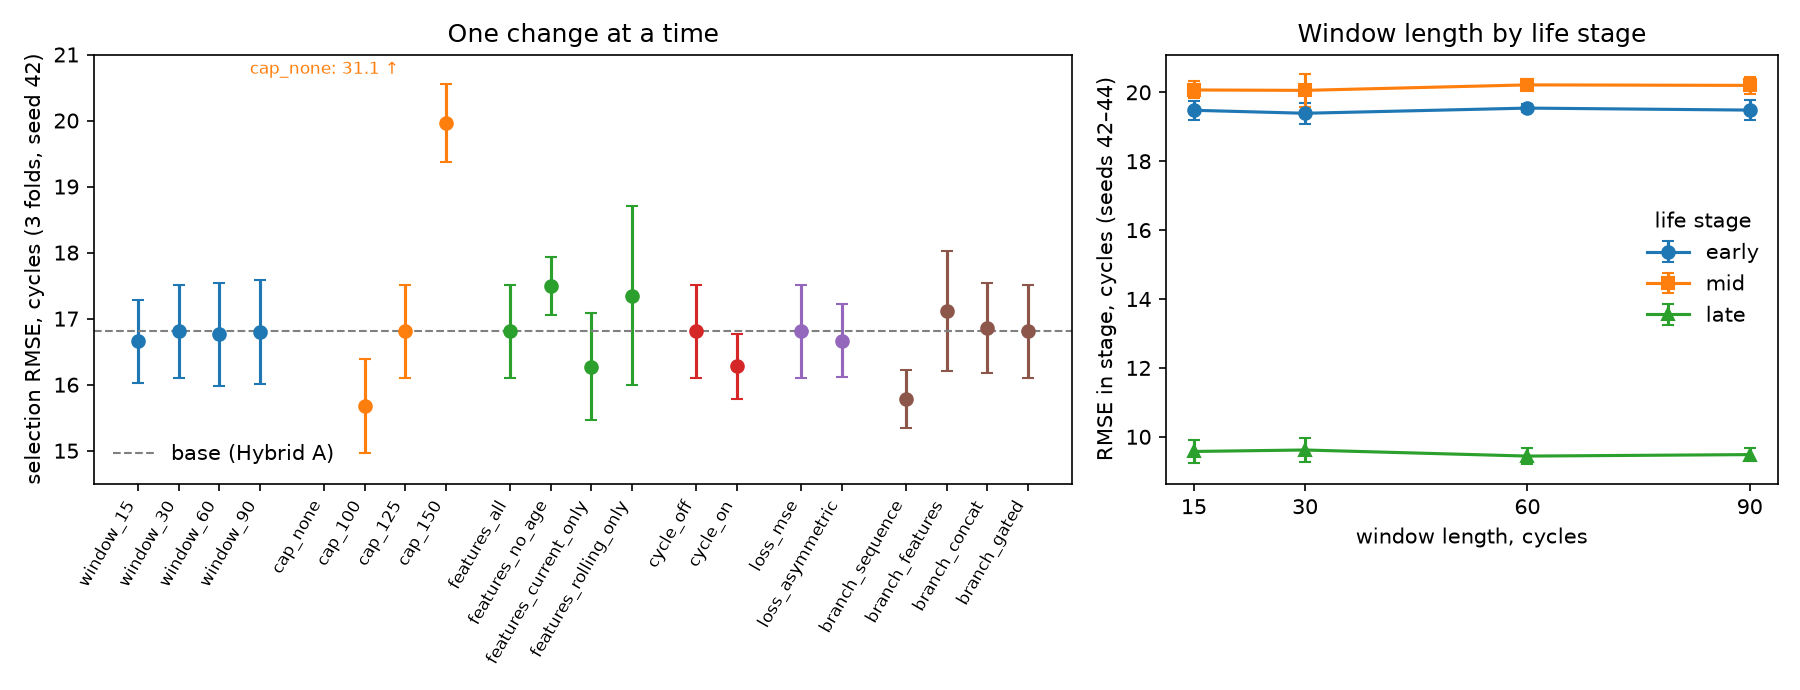
\includegraphics[width=\textwidth]{../../results/figures/fd001_ablations.png}
\caption{Left: selection RMSE of every variant (seed 42, mean $\pm$ s.d.\ over
folds); the dashed line is the base. ``No cap'' (31.1) is off the axis.
Right: RMSE by life stage against window length, mean $\pm$ s.d.\ over
seeds 42--44.}
\label{fig:ablations}
\end{figure*}

\subsection{Results}
Table~\ref{tab:ablations} and Fig.~\ref{fig:ablations} give the results.

\paragraph{Window length}
Longer history does not help Hybrid A on FD001. Windows of 15, 60 and 90
cycles score within 0.07 cycles of the 30-cycle base. Every interval lies
inside $\pm0.26$, and every corrected $p$ is 1. The answer holds at every
life stage (Fig.~\ref{fig:ablations}, right). Late-stage RMSE falls from
9.62 at 30 cycles to 9.44 at 60, which is smaller than the seed spread of
0.24--0.34. Two features of the setup may explain this, though neither was
tested here. The feature branch already summarizes the last 20 cycles, so
extra raw history may add little. FD001 also degrades slowly and smoothly
near failure. Chen et al.~\cite{Chen2021machine} found 30 to be the best
window for an FD001 LSTM, with longer windows worse; here longer windows are
no better but also no worse. Our result applies to this model and
subset. FD004, with two fault modes, could behave differently and is not
tested here.

\paragraph{Branches}
The gate makes the model more stable rather than clearly more accurate.
With only the sequence branch, a single seed looked 1.0 cycle \emph{better}
than the hybrid. Over three seeds it is 0.29 worse, an interval of $-1.49$
to $+2.19$, and its seed spread is four times larger (0.98 against 0.24).
This is why the group was repeated. The sequence branch alone is better in
the early stage (15.88 against 19.39) but worse in the late stage (11.10
against 9.62). The gate gives up some early-stage accuracy for accuracy near
failure, which matters most for maintenance. With only the feature branch,
the model is 0.79 worse. That interval excludes zero, but the corrected
$p$ is 0.051, so the evidence that the sequence branch adds information is
borderline. Plain concatenation is 0.31 worse ($-0.03$ to $+0.64$), so the
gate's own gain over joining the branches is small.

\paragraph{Training cap}
No cap and a cap of 150 are clearly worse, by 14.32 and 3.15 cycles (both
$p<0.001$). A cap of 100 is 1.13 better, but its interval reaches $+0.05$
and the difference is not significant. It is more accurate in the mid and
late stages (14.70 and 7.92 against 20.47 and 9.70) and less accurate in
the early stage (24.67 against 19.41). This repeats the tabular result of
Section~\ref{sec:target_selection}. The selection rule rules out 150 and no
cap, but it cannot separate 100 from 125. The result bears on that
section's caveat that the sequence models may prefer a different cap. At one
seed, Hybrid A leans toward 100 by 1.13 cycles, more than its seed spread,
but the difference is not significant. A multi-seed run would be needed to
settle it.

\paragraph{Feature groups and cycle index}
No change to the feature groups is significant: no age $+0.68$, rolling
statistics only $+0.56$, age and current sensors only $-0.53$. All three
intervals include zero. Together with the window result, this suggests the
hybrid does not depend on the rolling features, because the sequence branch
already sees recent history. Adding the cycle index to the sequence branch
changes RMSE by $-0.53$ ($-1.52$ to $+0.51$). The feature branch already
receives the engine's age, so the extra input is largely redundant.

\paragraph{Loss}
The asymmetric loss leaves RMSE unchanged ($-0.14$, $-0.80$ to $+0.50$)
but changes the direction of the errors. Over the selection band, the mean
signed error moves from $+0.62$ to $-0.45$ cycles. The NASA score falls by
12\% (from 127{,}571 to 112{,}268). The share of late predictions stays at
52\%. The loss therefore shrinks late errors rather than removing them.

\subsection{Conclusions and Limits}
No variant beats the base with statistical support, so Hybrid A keeps its
tuned settings for the final test run. The study answers the brief's question: on FD001,
longer history does not improve Hybrid A at any life stage. Three limits
apply. (i)~The cap, feature, cycle and loss groups use one seed. Their
differences of under one cycle are within the seed spread of the
sequence-only model. (ii)~Each variant changes a single setting, so
interactions are not tested, for example a longer window with the sequence
branch alone. (iii)~All results are on FD001. Regime normalization on
FD002 and FD004 is studied separately (issue~\#70).
